\def\leftcircle{(-1,0) circle (2 cm)}
\def\rightcircle{(1,0) circle (2 cm)}
\begin{figure}[H]
  \centering
  \label{tikzpic:set_union}
  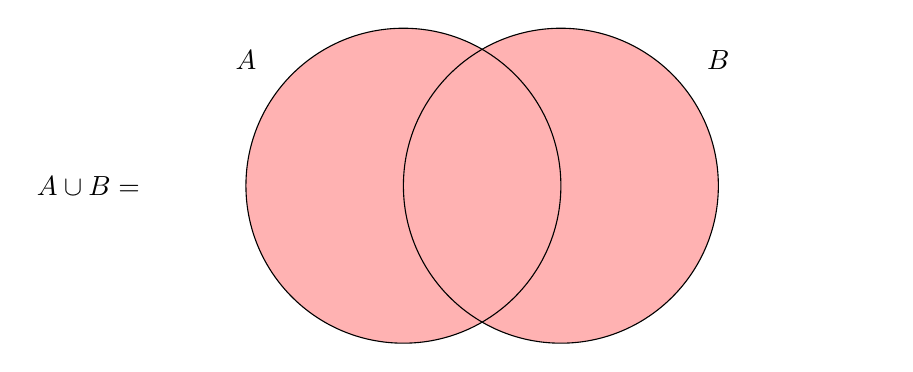
\begin{tikzpicture}
    \fill[red!30] \rightcircle;
    \fill[red!30] \leftcircle;

    \draw \leftcircle;
    \draw \rightcircle;
    \draw (-3,1.6) node {$A$};
    \draw (3,1.6) node {$B$};
    \draw (-5,0) node {$A \cup B = $};
    \draw (5,0) node {\text{     }};
  \end{tikzpicture}
  \caption{Объединение множеств}
\end{figure}

